\documentclass[12pt,a4paper]{article}

% =========================
% PAQUETES
% =========================
\usepackage[utf8]{inputenc}
\usepackage[T1]{fontenc}
\usepackage[spanish]{babel}
\usepackage{geometry}
\usepackage{graphicx}
\usepackage{float}
\usepackage{booktabs}
\usepackage{xcolor}
\usepackage{listings}
\usepackage{hyperref}
\usepackage{caption}
\usepackage{array}
\usepackage{enumitem}

\geometry{margin=2.5cm}

\hypersetup{
    colorlinks=true,
    linkcolor=black,
    urlcolor=blue,
    citecolor=black
}

% =========================
% CONFIGURACIÓN DE CÓDIGO
% =========================
\lstdefinestyle{javaStyle}{
    language=Java,
    basicstyle=\ttfamily\small,
    keywordstyle=\color{blue}\bfseries,
    commentstyle=\color{gray},
    stringstyle=\color{red!60!black},
    numbers=left,
    numberstyle=\tiny\color{gray},
    stepnumber=1,
    numbersep=8pt,
    breaklines=true,
    frame=single,
    tabsize=4,
    showstringspaces=false,
    captionpos=b
}

\lstset{style=javaStyle}

% =========================
% DATOS DEL DOCUMENTO
% =========================
\begin{document}

\noindent
\textbf{Nombre:} Andy Paul Sánchez Pilaloa\\
\textbf{Curso:} 7mo Software ``A''\\
\textbf{Asignatura:} Aplicaciones Distribuidas\\
\textbf{Fecha:} Martes, 2 de junio de 2026\\
\textbf{Título:} Implementación de un prototipo de RegistroDistribuido con sockets TCP, Lamport, heartbeats, Bully y autenticación por token\\
\textbf{Repositorio:} \url{https://github.com/AndySanchez2004/Aplicaciones-Distribuidas}

\vspace{0.5cm}

\tableofcontents
\newpage

% ==========================================================
\section{Introducción}
% ==========================================================

En esta práctica se desarrolló un prototipo llamado \textit{RegistroDistribuido}, con el objetivo de aplicar varios conceptos vistos en la Unidad 1 de Aplicaciones Distribuidas. El sistema fue implementado en Java usando sockets TCP y se ejecutó de forma local en IntelliJ IDEA mediante tres nodos: Nodo 1, Nodo 2 y Nodo 3, asociados a los puertos 9001, 9002 y 9003.

El prototipo permite que un cliente se conecte a un nodo, se autentique mediante un token y envíe operaciones tipo \texttt{MSG}. Además, cada nodo mantiene un contador lógico de Lamport, envía heartbeats a los demás nodos y detecta cuando alguno deja de responder. También se incluyó una aproximación al algoritmo Bully para representar la elección de coordinador.

La finalidad principal fue construir una demostración funcional, pequeña y entendible, donde se evidencien comunicación entre procesos, sincronización lógica, tolerancia a fallos, coordinación y seguridad básica.

% ==========================================================
\section{Objetivos}
% ==========================================================

\subsection{Objetivo general}

Implementar un prototipo distribuido en Java que demuestre comunicación TCP, reloj lógico de Lamport, heartbeats, detección de fallos, coordinación básica con Bully y autenticación por token.

\subsection{Objetivos específicos}

\begin{itemize}
    \item Crear un cliente TCP capaz de conectarse a un nodo y enviar operaciones.
    \item Ejecutar tres nodos locales en puertos diferentes.
    \item Validar un token antes de aceptar la comunicación del cliente.
    \item Incrementar un reloj lógico cada vez que se recibe una operación.
    \item Enviar heartbeats entre nodos para detectar fallos.
    \item Registrar evidencias de ejecución mediante capturas de pantalla.
\end{itemize}

% ==========================================================
\section{Materiales y métodos}
% ==========================================================

\subsection{Entorno de desarrollo}

El prototipo fue realizado en Java desde IntelliJ IDEA, usando Maven como estructura base del proyecto. La ejecución se hizo localmente, utilizando diferentes puertos para simular varios nodos en una misma máquina.

\begin{table}[H]
\centering
\caption{Herramientas utilizadas}
\begin{tabular}{ll}
\toprule
\textbf{Elemento} & \textbf{Detalle} \\
\midrule
Lenguaje & Java \\
IDE & IntelliJ IDEA \\
Proyecto & Maven \\
Comunicación & Sockets TCP \\
Ejecución & Localhost \\
Puertos & 9001, 9002 y 9003 \\
\bottomrule
\end{tabular}
\end{table}

\subsection{Creación del proyecto}

El proyecto se creó en IntelliJ IDEA desde la opción \textit{File} $\rightarrow$ \textit{New} $\rightarrow$ \textit{Project}, seleccionando el arquetipo \texttt{maven-archetype-quickstart}. La configuración usada fue:

\begin{table}[H]
\centering
\caption{Configuración inicial del proyecto}
\begin{tabular}{ll}
\toprule
\textbf{Parámetro} & \textbf{Valor} \\
\midrule
Nombre & \texttt{servidor-tcp} \\
GroupId & \texttt{ec.edu.uteq.distribuidas} \\
ArtifactId & \texttt{servidor-tcp} \\
Arquetipo & \texttt{maven-archetype-quickstart} \\
\bottomrule
\end{tabular}
\end{table}

Dentro del paquete principal se trabajó con dos clases principales: \texttt{Cliente.java}, encargada de conectarse y enviar operaciones, y \texttt{NodoDistribuido.java}, encargada de funcionar como nodo servidor, manejar mensajes, enviar heartbeats y detectar fallos.

\begin{figure}[H]
    \centering
    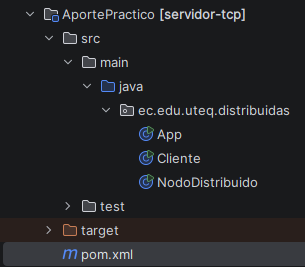
\includegraphics[width=0.55\textwidth]{imagenes/figura1_estructura_proyecto.png}
    \caption{Estructura del proyecto en IntelliJ IDEA.}
    \label{fig:estructura-proyecto}
\end{figure}

% ==========================================================
\section{Desarrollo de la implementación}
% ==========================================================

\subsection{Parte A --- Comunicación entre procesos}

La comunicación se realizó con sockets TCP. El cliente se conecta al Nodo 1 mediante \texttt{localhost} y el puerto \texttt{9001}. Para enviar mensajes se usó \texttt{PrintWriter}, y para recibir respuestas se usó \texttt{BufferedReader}.

\begin{lstlisting}[caption={Conexión TCP del cliente.}]
Socket socket = new Socket("localhost", 9001);
BufferedReader in = new BufferedReader(
        new InputStreamReader(socket.getInputStream()));
PrintWriter out = new PrintWriter(socket.getOutputStream(), true);
Scanner sc = new Scanner(System.in);
\end{lstlisting}

Los mensajes se delimitan con saltos de línea, usando \texttt{println()} para enviar y \texttt{readLine()} para recibir. Esto permite que cada mensaje sea procesado de forma individual.

\begin{lstlisting}[caption={Envío y recepción de mensajes desde el cliente.}]
while (true) {
    System.out.print("> ");
    String msg = sc.nextLine();

    out.println(msg);
    System.out.println(in.readLine());
}
\end{lstlisting}

En cada nodo se levanta un servidor TCP. Cuando llega una conexión, se crea un hilo para atenderla sin bloquear al resto del sistema.

\begin{lstlisting}[caption={Servidor TCP del nodo distribuido.}]
private void server() {
    try (ServerSocket ss = new ServerSocket(puerto)) {
        while (true) {
            Socket socket = ss.accept();
            new Thread(() -> handle(socket)).start();
        }
    } catch (Exception e) {
        e.printStackTrace();
    }
}
\end{lstlisting}

\begin{figure}[H]
    \centering
    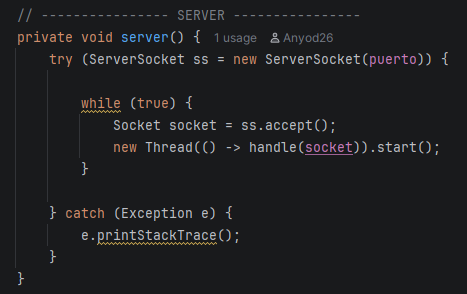
\includegraphics[width=0.95\textwidth]{imagenes/figura2_servidor_tcp.png}
    \caption{Inicio del nodo distribuido y servidor TCP.}
    \label{fig:servidor-tcp}
\end{figure}

\subsection{Parte B --- Reloj lógico de Lamport}

Cada nodo tiene una variable llamada \texttt{relojLamport}. Cuando el nodo recibe un mensaje que empieza con \texttt{MSG}, incrementa el contador y responde con un ACK que incluye el valor actual del reloj.

\begin{lstlisting}[caption={Actualización del reloj lógico de Lamport.}]
if (msg.startsWith("MSG")) {
    relojLamport++;
    out.println("NODO " + id + " ACK Lamport=" + relojLamport);
}
\end{lstlisting}

En esta versión se aplicó el incremento local del reloj. Para una versión más completa, los mensajes entre nodos deberían incluir también la marca lógica del emisor y aplicar la regla \texttt{max(local, recibido) + 1}.

\begin{figure}[H]
    \centering
    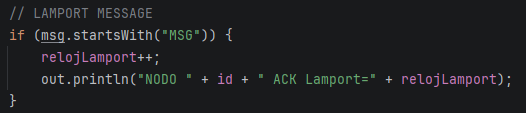
\includegraphics[width=0.90\textwidth]{imagenes/figura3_lamport_codigo.png}
    \caption{Procesamiento de operaciones con reloj Lamport.}
    \label{fig:lamport-codigo}
\end{figure}

\subsection{Parte C --- Heartbeats y detección de fallos}

Cada nodo ejecuta una tarea periódica que intenta comunicarse con los demás nodos cada tres segundos. Si un nodo no responde, se registra como caído.

\begin{lstlisting}[caption={Envío periódico de heartbeats.}]
private void heartbeatTask() {
    while (true) {
        try {
            Thread.sleep(3000);

            for (int nodo : puertos.keySet()) {
                if (nodo != id) {
                    send(nodo, "HB");
                }
            }
        } catch (Exception ignored) {}
    }
}
\end{lstlisting}

La detección del fallo ocurre dentro del método \texttt{send}. Si la conexión TCP no se puede establecer, el nodo imprime en consola qué nodo fue detectado como caído.

\begin{lstlisting}[caption={Registro de nodo caído.}]
catch (Exception e) {
    System.out.println("Nodo " + nodo + " caído detectado por " + id);
    nodosActivos.remove(nodo);
}
\end{lstlisting}

\begin{figure}[H]
    \centering
    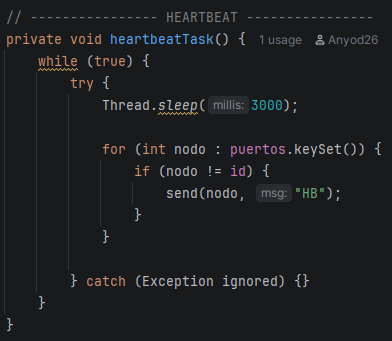
\includegraphics[width=0.95\textwidth]{imagenes/figura4_heartbeat_fallos.png}
    \caption{Heartbeat y detección de nodos caídos.}
    \label{fig:heartbeat-fallos}
\end{figure}

\subsection{Parte D --- Coordinación con Bully}

El Nodo 3 se definió como coordinador inicial, porque tiene el identificador más alto. Esta idea sigue el principio del algoritmo Bully, donde el nodo activo con mayor ID debe actuar como líder.

\begin{lstlisting}[caption={Coordinador inicial.}]
if (id == 3) {
    coordinador.set(true);
    System.out.println("Nodo " + id + " es COORDINADOR inicial");
}
\end{lstlisting}

También se incluyó un método de elección para iniciar el proceso cuando se detecta la caída del coordinador.

\begin{lstlisting}[caption={Inicio de elección de coordinador.}]
private void startElection() {
    System.out.println("Nodo " + id + " inicia ELECTION");

    for (int nodo : nodosActivos) {
        if (nodo > id) {
            send(nodo, "ELECTION");
        }
    }

    coordinador.set(true);
    System.out.println("Nodo " + id + " es nuevo COORDINADOR");
}
\end{lstlisting}

La implementación representa una versión básica del algoritmo. En una versión más robusta, el nodo debería esperar respuestas \texttt{OK} antes de declararse coordinador.

\begin{figure}[H]
    \centering
    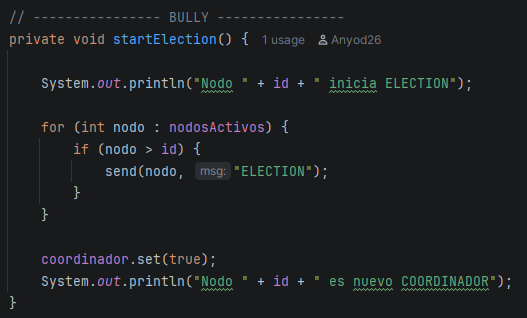
\includegraphics[width=0.95\textwidth]{imagenes/figura5_bully_codigo.png}
    \caption{Método de elección de coordinador.}
    \label{fig:bully}
\end{figure}

\subsection{Parte E --- Seguridad por token}

Antes de enviar operaciones, el cliente manda el token \texttt{TOKEN:123}. El nodo lo valida y responde \texttt{OK AUTH} si es correcto o \texttt{TOKEN INVALIDO} si no coincide.

\begin{lstlisting}[caption={Validación del token.}]
if (msg.startsWith("TOKEN:")) {
    if (!msg.split(":")[1].equals("123")) {
        out.println("TOKEN INVALIDO");
        continue;
    }
    out.println("OK AUTH");
    continue;
}
\end{lstlisting}

Este mecanismo no reemplaza una seguridad real con cifrado o sesiones, pero sí permite demostrar una autenticación básica antes de aceptar operaciones.

% ==========================================================
\section{Resultados obtenidos}
% ==========================================================

\subsection{Ejecución de nodos}

Se ejecutaron tres instancias de \texttt{NodoDistribuido}. Cada una usó un identificador y puerto diferente.

\begin{table}[H]
\centering
\caption{Nodos ejecutados}
\begin{tabular}{ccc}
\toprule
\textbf{Nodo} & \textbf{ID} & \textbf{Puerto} \\
\midrule
Nodo 1 & 1 & 9001 \\
Nodo 2 & 2 & 9002 \\
Nodo 3 & 3 & 9003 \\
\bottomrule
\end{tabular}
\end{table}

\begin{figure}[H]
    \centering
    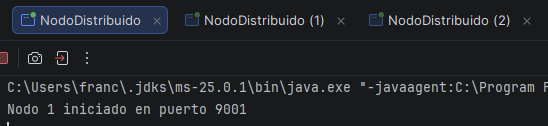
\includegraphics[width=0.90\textwidth]{imagenes/figura6_nodo1_iniciado.png}
    \caption{Nodo 1 iniciado en el puerto 9001.}
    \label{fig:nodo1}
\end{figure}

\begin{figure}[H]
    \centering
    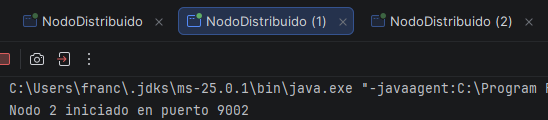
\includegraphics[width=0.90\textwidth]{imagenes/figura7_nodo2_iniciado.png}
    \caption{Nodo 2 iniciado en el puerto 9002.}
    \label{fig:nodo2}
\end{figure}

\begin{figure}[H]
    \centering
    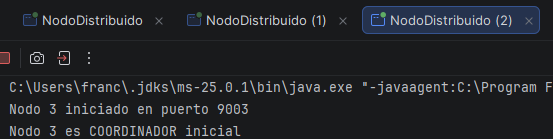
\includegraphics[width=0.90\textwidth]{imagenes/figura8_nodo3_coordinador.png}
    \caption{Nodo 3 iniciado como coordinador inicial.}
    \label{fig:nodo3}
\end{figure}

Como se observa, los tres nodos iniciaron correctamente. El Nodo 3 asumió el rol de coordinador inicial.

\subsection{Cliente autenticado y operaciones}

El cliente se conectó al Nodo 1, envió el token y recibió la respuesta \texttt{OK AUTH}. Luego se enviaron operaciones tipo \texttt{MSG}, recibiendo respuestas con el valor del reloj Lamport.

\begin{figure}[H]
    \centering
    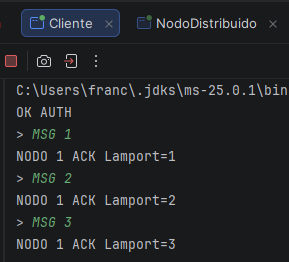
\includegraphics[width=0.90\textwidth]{imagenes/figura9_cliente_lamport.png}
    \caption{Cliente autenticado y operaciones con Lamport.}
    \label{fig:cliente-lamport}
\end{figure}

También se registró una prueba adicional de comportamiento con fallo durante la comunicación del cliente.

\begin{figure}[H]
    \centering
    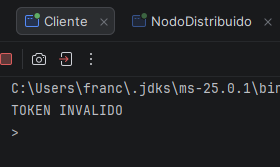
\includegraphics[width=0.90\textwidth]{imagenes/figura9_cliente_lamport_fallo.png}
    \caption{Evidencia adicional de comunicación del cliente durante la prueba.}
    \label{fig:cliente-lamport-fallo}
\end{figure}

\subsection{Detección de fallos}

Los nodos registraron en consola cuando otro nodo dejó de responder. Esta evidencia confirma que el mecanismo de heartbeats permitió detectar fallos parciales.

\begin{figure}[H]
    \centering
    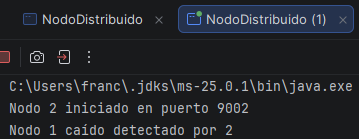
\includegraphics[width=0.90\textwidth]{imagenes/figura10_fallo_nodo1.png}
    \caption{Detección de fallos desde el Nodo 1.}
    \label{fig:fallo-nodo1}
\end{figure}

\begin{figure}[H]
    \centering
    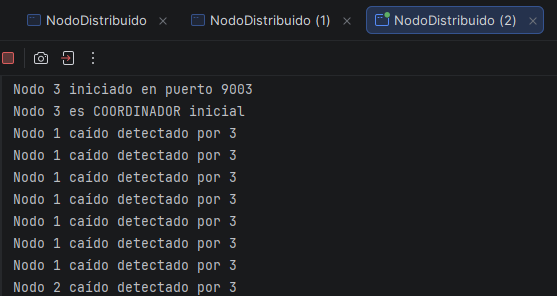
\includegraphics[width=0.90\textwidth]{imagenes/figura11_fallo_nodo2.png}
    \caption{Detección de fallos desde el Nodo 2.}
    \label{fig:fallo-nodo2}
\end{figure}

\begin{figure}[H]
    \centering
    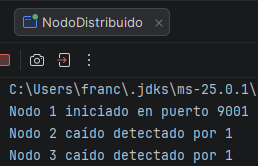
\includegraphics[width=0.90\textwidth]{imagenes/figura12_fallo_nodo3.png}
    \caption{Detección de fallos desde el Nodo 3.}
    \label{fig:fallo-nodo3}
\end{figure}

% ==========================================================
\section{Análisis técnico}
% ==========================================================

\subsection{Compromiso CAP}

El prototipo prioriza la disponibilidad y la tolerancia a fallos parciales. Cuando un nodo deja de responder, los demás continúan activos y registran la caída en consola. Sin embargo, no se garantiza consistencia fuerte, porque las operaciones no se replican en todos los nodos ni existe un consenso antes de responder al cliente.

Por esta razón, el comportamiento se acerca más a un enfoque AP: el sistema intenta seguir funcionando aunque existan fallos de comunicación. Para lograr un modelo CP sería necesario bloquear operaciones o usar un algoritmo de consenso antes de confirmar cada registro.

\subsection{Falacias de la computación distribuida consideradas}

Durante la práctica se evidenció que la red no siempre es confiable, ya que un nodo puede dejar de responder y generar una excepción de conexión. También se consideró que la latencia no es cero, por eso los heartbeats se ejecutan cada cierto intervalo y no de forma instantánea.

Otra falacia considerada fue asumir que la red es segura. Para evitar que cualquier cliente envíe operaciones sin control, se agregó una autenticación básica mediante token. Además, como TCP trabaja como flujo de bytes, los mensajes se delimitaron con saltos de línea usando \texttt{println()} y \texttt{readLine()}.

\subsection{Transparencias ofrecidas}

La solución ofrece una transparencia de acceso parcial, porque el cliente solo envía mensajes y recibe respuestas sin conocer todo el procesamiento interno del nodo. También existe una transparencia de fallos limitada, ya que los nodos detectan caídas mediante heartbeats.

No se ofrece transparencia de ubicación completa, porque el cliente conoce directamente el puerto \texttt{9001}. Tampoco existe transparencia de replicación completa, ya que las operaciones no se copian automáticamente entre todos los nodos.

\subsection{SLA propuesto}

Para este prototipo se propone un SLA de disponibilidad del 99.9\%. Esto permite calcular el tiempo máximo de inactividad anual con la siguiente fórmula:

\[
T_{\text{caída}} = (1 - D) \times T_{\text{total}}
\]

Donde:

\[
D = 0.999
\]

\[
T_{\text{total}} = 8760 \text{ horas/año}
\]

Entonces:

\[
T_{\text{caída}} = (1 - 0.999) \times 8760 = 8.76 \text{ horas/año}
\]

Por tanto, con un SLA del 99.9\%, el sistema podría estar inactivo aproximadamente 8.76 horas al año. Si el SLA fuera de 99.99\%, el tiempo de caída bajaría a aproximadamente 52.6 minutos anuales.

\subsection{Comparación con Raft}

Si se reemplazara Bully por Raft, el sistema tendría una elección de líder más robusta y podría mantener un log replicado entre nodos. Esto ayudaría a mejorar la consistencia de las operaciones.

El costo sería una mayor complejidad, más mensajes entre nodos y mayor latencia antes de confirmar una operación. Para esta práctica, Bully fue suficiente para representar la coordinación básica; para un sistema real, Raft sería más adecuado.

% ==========================================================
\section{Conclusiones}
% ==========================================================

Se logró implementar un prototipo distribuido en Java usando sockets TCP, con un cliente y tres nodos ejecutados localmente en los puertos 9001, 9002 y 9003. La comunicación funcionó mediante mensajes delimitados por salto de línea, permitiendo enviar operaciones y recibir respuestas desde consola.

También se incorporó autenticación básica por token. El cliente envía \texttt{TOKEN:123} y el nodo responde \texttt{OK AUTH} cuando la validación es correcta. Esto permitió demostrar un control inicial antes de aceptar operaciones.

El reloj lógico de Lamport se aplicó mediante un contador que aumenta cada vez que el nodo recibe una operación \texttt{MSG}. Aunque la implementación puede mejorar incorporando la regla completa \texttt{max(local, recibido) + 1}, el prototipo permitió observar el avance lógico de los eventos.

Finalmente, los heartbeats permitieron detectar nodos caídos durante la ejecución. El Nodo 3 fue definido como coordinador inicial y se agregó una versión básica del algoritmo Bully para representar la elección de líder.

% ==========================================================
\newpage
\section{Anexos}
% ==========================================================

\subsection{Código completo de Cliente.java}

\begin{lstlisting}[caption={Código completo de Cliente.java}]
package ec.edu.uteq.distribuidas;

import java.io.*;
import java.net.*;
import java.util.Scanner;

public class Cliente {

    public static void main(String[] args) {

        try (
                Socket socket = new Socket("localhost", 9001);
                BufferedReader in = new BufferedReader(new InputStreamReader(socket.getInputStream()));
                PrintWriter out = new PrintWriter(socket.getOutputStream(), true);
                Scanner sc = new Scanner(System.in)
        ) {

            // AUTH
            out.println("TOKEN:123");
            System.out.println(in.readLine());

            while (true) {

                System.out.print("> ");
                String msg = sc.nextLine();

                out.println(msg);

                System.out.println(in.readLine());
            }

        } catch (Exception e) {
            e.printStackTrace();
        }
    }
}
\end{lstlisting}

\subsection{Código completo de NodoDistribuido.java}

\begin{lstlisting}[caption={Código completo de NodoDistribuido.java}]
package ec.edu.uteq.distribuidas;

import java.io.*;
import java.net.*;
import java.util.*;
import java.util.concurrent.*;
import java.util.concurrent.atomic.AtomicBoolean;

public class NodoDistribuido {

    private final int id;
    private final int puerto;

    private int relojLamport = 0;

    private final Set<Integer> nodosActivos = new HashSet<>();
    private final Map<Integer, Integer> puertos = new HashMap<>();

    private final AtomicBoolean coordinador = new AtomicBoolean(false);
    private volatile boolean activo = true;

    public NodoDistribuido(int id, int puerto) {
        this.id = id;
        this.puerto = puerto;

        puertos.put(1, 9001);
        puertos.put(2, 9002);
        puertos.put(3, 9003);

        nodosActivos.add(1);
        nodosActivos.add(2);
        nodosActivos.add(3);
    }

    public static void main(String[] args) {
        if (args.length < 2) {
            System.err.println("Error: Faltan argumentos.");
            System.err.println("Uso: java NodoDistribuido <id_nodo> <puerto>");
            System.exit(1);
        }

        int id = Integer.parseInt(args[0]);
        int puerto = Integer.parseInt(args[1]);

        new NodoDistribuido(id, puerto).start();
    }

    public void start() {
        System.out.println("Nodo " + id + " iniciado en puerto " + puerto);

        Executors.newSingleThreadExecutor().submit(this::heartbeatTask);

        Executors.newSingleThreadExecutor().submit(this::server);

        if (id == 3) {
            coordinador.set(true);
            System.out.println("Nodo " + id + " es COORDINADOR inicial");
        }
    }

    private void server() {
        try (ServerSocket ss = new ServerSocket(puerto)) {

            while (true) {
                Socket socket = ss.accept();
                new Thread(() -> handle(socket)).start();
            }

        } catch (Exception e) {
            e.printStackTrace();
        }
    }

    private void handle(Socket socket) {
        try (
                BufferedReader in = new BufferedReader(new InputStreamReader(socket.getInputStream()));
                PrintWriter out = new PrintWriter(socket.getOutputStream(), true)
        ) {

            String msg;

            while ((msg = in.readLine()) != null) {

                if (msg.startsWith("TOKEN:")) {
                    if (!msg.split(":")[1].equals("123")) {
                        out.println("TOKEN INVALIDO");
                        continue;
                    }
                    out.println("OK AUTH");
                    continue;
                }

                if (msg.startsWith("MSG")) {
                    relojLamport++;
                    out.println("NODO " + id + " ACK Lamport=" + relojLamport);
                }

                if (msg.equals("HB")) {
                    nodosActivos.add(1);
                }

                if (msg.equals("ELECTION")) {
                    if (id > 1) {
                        out.println("OK");
                    }
                }

                if (msg.equals("COORDINATOR")) {
                    coordinador.set(true);
                }
            }

        } catch (Exception e) {
            System.out.println("Nodo " + id + " caído cliente");
        }
    }

    private void heartbeatTask() {
        while (true) {
            try {
                Thread.sleep(3000);

                for (int nodo : puertos.keySet()) {
                    if (nodo != id) {
                        send(nodo, "HB");
                    }
                }

            } catch (Exception ignored) {}
        }
    }

    private void send(int nodo, String msg) {
        try (Socket s = new Socket("localhost", puertos.get(nodo));
             PrintWriter out = new PrintWriter(s.getOutputStream(), true)) {

            out.println(msg);

        } catch (Exception e) {
            System.out.println("Nodo " + nodo + " caído detectado por " + id);

            nodosActivos.remove(nodo);

            if (coordinador.get() && nodo == 3) {
                startElection();
            }
        }
    }

    private void startElection() {

        System.out.println("Nodo " + id + " inicia ELECTION");

        for (int nodo : nodosActivos) {
            if (nodo > id) {
                send(nodo, "ELECTION");
            }
        }

        coordinador.set(true);
        System.out.println("Nodo " + id + " es nuevo COORDINADOR");
    }
}
\end{lstlisting}

\end{document}